\chapter{Il problema della selezione e le statistiche d'ordine}
\colorbox{SALZO}{\parbox{\dimexpr\linewidth-2\fboxsep}{\begin{definition}
    Statistica d'ordine\\
    Dato un insieme A di n numeri (distinti), la k-esima statistica d'ordine è il k-esimo elemento più piccolo di A.\\
    \begin{itemize} 
        \item il minimo di un insieme A è la prima statistica d'ordine.
        \item il massimo di un insieme A è l'n-esima statistica d'ordine.
        \item la mediana di un insieme A è l'elemento di mezzo.\\
        - se dispari una mediana $\lfloor (n+1)/2 \rfloor$.\\
        - se pari due mediana una inferiore e una superiore $\lceil (n+1)/2 \rceil$.
\end{itemize}
    
\end{definition}}}\medskip\\ 

\section{Problema selezione}
Dato un insieme di elementi A il problema della selezione consiste nel selezionare la k-esima statistica d'ordine.\\
definiamo il \textbf{problema della selezione} come segue:
\textbf{input: }un insieme A di n numeri (distinti) ed un intero k, con $ 1 \le k \le n $.
\textbf{output: } $x \in A$ tale che x è il k-esimo in ordine di grandezza.\\
osservazione:\\
dato un elemento $x \in A$, x è il k-esimo in ordine di grandezza se gli altri n-1 elementi si possono ripartire in 2 gruppi tali che:
\begin{itemize}
    \item un gruppo contiene k-1 elementi tutti minori o uguali di x ed
    \item un gruppo contiene n-k elementi tutti maggiori o uguali di x
\end{itemize}

\section{Minimo o Massimo}
Trovare il minimo e il massimo di un insieme sono problemi molto comuni e per cui già conosciamo un algoritmo semplice: 
\begin{verbatim}
1    Minium(a,n)
2        min=A[1]
3        for i=2 to n
4            if min > A[j]
5                min = A[i]
6        return min
\end{verbatim}
\textbf{osservazioni}
n-1 confronti è un upper bound per il problema del minimo/massimo\\
L'algoritmo proposto è ottimo rispetto al numero di confronti e la complessità è $\Theta(n)$

\section{Minimo e Massimo}
Come sappiamo per cercare il min o il max siamo abituati a svolgere n confronti, ovvero confrontare ciascun elemento dell'array con il min e max.  \\ 
Per trovare sia il minimo che il massimo, eseguo in sequenza Minium e il duale Maxium (soluzione Naif) e ottengo un totale di 2(n-1) confronti.
Il costo asintotico nel caso peggiore per la ricerca del min e del max è $\Theta(n)$, non è possibile trovare un algoritmo che faccia meglio. Nonostante ciò, è comunque possibile scansionarli a coppie così che il numero di cicli passi da n a $\frac{n}{2}$ e con al più $3 \lfloor n/2 \rfloor $.\\
\subsection{Psudocodice}
\begin{verbatim}
1    Min-Max(A,n)
2    if (n è dispari) then
3        max=A[1];
4        min=A[1];
5        i=2;
6    else
7        if(A[1]<A[2]) then
8            max=A[2];
9            min=A[1];
10            i=3;
11        else
12            max=A[1];
13            min=A[2];
14            i=3;
15        end
16    end
17    while(i<n) do
18        if(A[i]<A[i+1]) then
19            if (A[i]<min) then
20                min=A[i];
21            end
22            if (A[i+1]>max) then
23                max=A[i+1];
24            end
25        else
26            if(A[i+1]<min) then
27                min=A[i+1];
28            end
29            if(A[i]>max) then
30                max=A[i];
31            end
32        end
33        i=i+2;
34    end
35    return min,max      
\end{verbatim}
\noindent Prima confrontiamo due elementi di input l'uno con l'altro e poi il più piccolo dei due con il minimo corrente, e il più grande dei due con il massimo corrente, con un costo di 3 confronti ogni 2 elementi.\\
Come si debba impostare i valori iniziali del minimo e del massimo dipende dal fatto che n sia pari o dispari. Se n è dispari, assegniamo al minimo e al massimo il valore del primo elemento, e poi esaminiamo i restanti elementi a coppie. Se n è pari, effettuiamo un confronto fra i primi 2 elementi per determinare i valori iniziali del minimo e del massimo; poi esaminiamo i restanti elementi a coppie, come nel caso di n dispari.\\
Nelle ietrazioni del ciclo while vengono effettuati sempre 3 confronti, allora è possibile dire che il numero di confronti se n è pari o dispari è:\\
$n$ dispari: $3 \cdot (\frac{n-1}{2})$ \qquad $n$ pari: $3 \cdot (\frac{n-2}{n})+1$\\
Nel caso di $n$ dispari viene assegnato ad $i$ il valore 2, questo significa che il while farà $\frac{n-1}{2}$ cicli; infatti, bisogna notare come $i$ venga incrementato di 2 ogni volta, dimezzando così il numeoro di cicli. 
Il tutto è moltiplicato per 3 in quanto come abbiamo visto il numero di confronti per il ciclo è 3. 
Nel caso $n$ pari dobbiamo considerare il costo costante del confronto (+1) e notare in seguito come ad $i$ venga assegnato il valore 3. 
Questo significa che, ragionando come prima, il numero di cicli che effettuerà il while sarà $\frac{n-2}{2}$, il tutto moltiplicato per 3 dato il numero di confronti per ciclo.\smallskip\\
\noindent \textit{Esempio.}\\
$A = <5,8,23,1,7,9>$ con $n=6$\\
\textbf{Passo 1:}\\
$n$ è pari allora prendo i primi due valori dell'array e li confronto e assegno $min=5$ e $max=8$ e pongo $i=3$\\
\textbf{Passo 2:}\\
\textbf{Iterazione 1:}
\begin{enumerate}
\item prendo la coppia $A[i] = 23$ e $A[i+1] = 1$:
\item $A[i] < A[i+1]$ ? No, allora:
\item $A[i+1]$ $<$ $min = 5$ ? Si, allora $min = 1$
\item $A[i]$ $>$ $max = 8$ ? Si, allora $max = 23$
\item $i = 3 + 2 = 5$
\end{enumerate}
\textbf{Iterazione 2:}
\begin{enumerate}
\item prendo la coppia A[i] = 7 e A[i+1] = 9:
\item $A[i]$ $<$ $A[i+1]$ ? Si, allora:
\item $A[i]$ $<$ $min = 1$ ? No
\item $A[i+1]$ $>$ $max = 23$ ? No
\item $i = 5 + 2 = 7$
\item esce dal ciclo e il programma termina con $min=1$ e $max=23$.
\end{enumerate}
\textit{Analisi esempio}.\\
\begin{figure}[H]
    \centering
    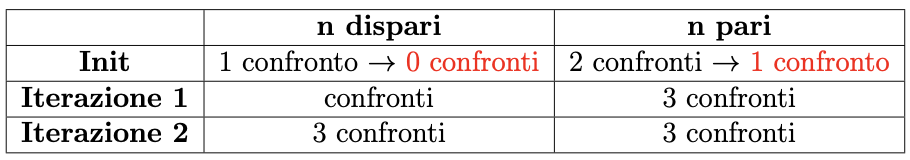
\includegraphics[width=0.5\linewidth]{../images/Screenshot 2026-03-22 alle 12.05.41.png}
    \label{fig:placeholder}
\end{figure}
\noindent 

\section{Selezione Randomizzata}
Il problema generale della selezione e il problema del minimo o del massimo hanno lo stesso tempo di esecuzione asintotico: $\Theta(n)$.
Sfruttiamo la proprietà della funzione partizione usata nel QuickSort e continuo a cercare solo se il pivot non è la statistica d'ordine che cercavo.\\
in dettaglio:\\
\begin{itemize}
    \item usiamo la versione modificata della procedura usata in QuickSort in cui il pivot viene scelto in modo casuale
    \item partizioniamo l'input come facciamo in QuickSort
    \item controllo in che posizione cade il pivot dopo la partizione
    \begin{itemize}[label=--]
        \item Se il pivot è nella posizione i corrispondente alla statistica d'ordine che cercavo ho finito
        \item Altrimenti faccio una chiamata ricorsiva su una sola delle due partizioni 
        \item Quale partizione scegliere per fare la chiamata ricorsiva dipende dalla relazione tra il pivot trovato e la mia statistica d'ordine cercata
    \end{itemize}
\end{itemize}
\noindent 
\subsection{Pseudocodice}
\begin{verbatim}
1   Randomized_Selecet(A,p,r,i)
2   if(p == r) then
3       return A[p]
4   end
5   q = Randomized_Partition(A,p,r)
6   k = q - p + 1
7   if(i == k)
8       return A[q]
9   else 
10     if (i < k) then  
11          return Randomized_Selecet(A,p,q-1,i);
12     else
13          return Randomized_Selecet(A,q+1,r,i-k);
14     end
15  end

16  Randomized_Partition(A,p,r)
17  i = random(p,r);
18  scambia(A[r],A[i]);
19  return partiziona(A,p,r) //stessa procedura usata in QuickSort
\end{verbatim}
\noindent 
\textit{Esempio.}\\
\begin{figure}[H]
    \centering
    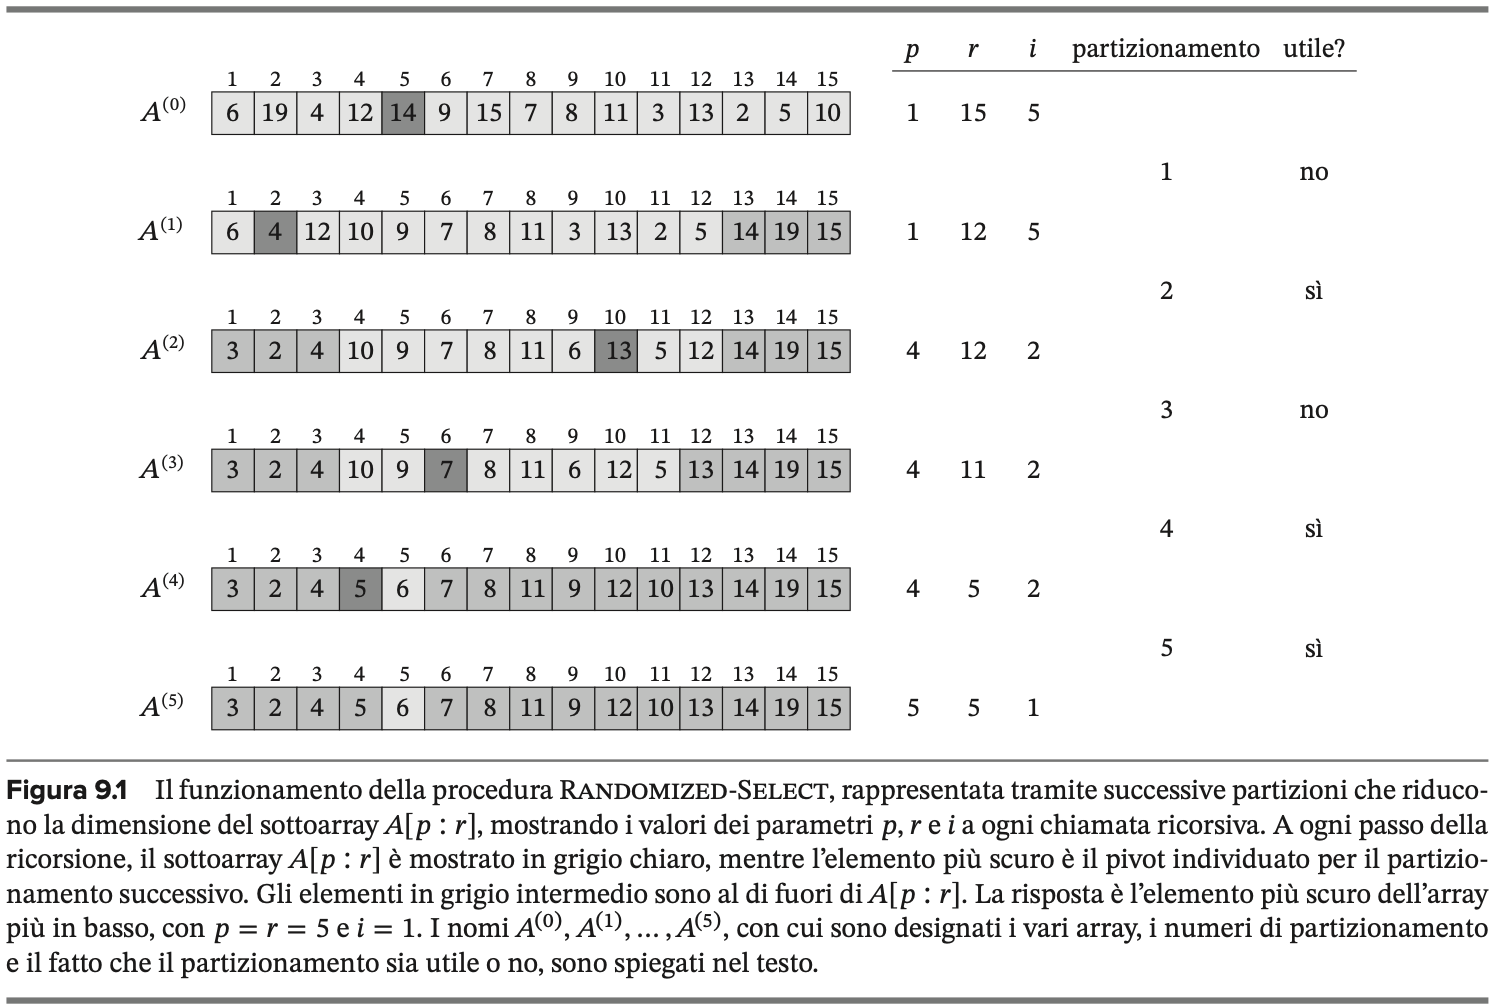
\includegraphics[width=0.75\linewidth]{../images/Screenshot 2026-03-22 alle 19.12.01.png}
    \label{fig:placeholder}
\end{figure}
\noindent \subsection{Analisi del costo}
Questo algoritmo ha un costo di caso peggiore $\Theta(n^2)$. poichè il partizionamento richiede un tempo $\Theta(n)$, la ricorrena per il tempo di esecuzione nel caso peggiore è la stessa di quella per QuickSort, ovvero $T(n)=T(n-1)*\Theta(n)$, che ha soluzione $T(n)=\Theta(n^2)$.Tuttavia la randomizzazione mi aiuta nel caso medio in cui il tempo atteso di esecuzione è lineare.\\
\subsection{Analisi del valore atteso del tempo di esecuzione}
\begin{figure}[H]
    \centering
    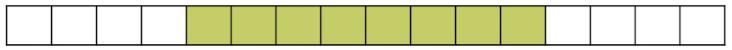
\includegraphics[width=0.5\linewidth]{../images/Screenshot 2026-03-23 alle 15.54.59.png}
    \label{fig:placeholder}
\end{figure}
\noindent Supponiamo che ogni volta che l'algoritmo seleziona casualmente un pivot, questo si trovi da qualche parte tra il secondo e il terzo quartile (parte centrale, quella in verde) degli elementi rimanenti, se presi in ordine.\\ Se l'i-esimo elemento più piccolo è minore del pivot, tutti gli elementi maggiori del pivot vengono ignorati in tutte le future chiamate ricorsive. Tra questi elementi che verranno sempre ignorati, ci sono senz'altro quelli del quartile superiore, e possibilmente anche qualcun altro. Allo stesso modo, se l'i-esimo elemento più piccolo è maggiore del pivot, tutti gli elementi minori del pivot, cioè almeno tutti quelli nel primo quartile, vengono ignorati in tutte le future chiamate ricorsive. \\
In entrambi i casi almeno $\frac{1}{4}$ degli elementi rimanenti viene ignorato in tutte le future chiamate ricorsive, lasciando in gioco al massimo $\frac{3}{4}$ degli elementi rimanenti, che rimarranno nell'array A[p : r]. Poiché Randomized-Partition richiede un tempo $\Theta(n)$ su un sottoarray di n elementi, la ricorrenza per il tempo di esecuzione nel caso peggiore è $T(n)=T(\frac{3n}{4})+\Theta(n)$; questa ricorrenza ha soluzione $T(n)=\Theta(n)$.\\
naturalmente il pivot non cade necessariamente ogni volta nella metà centrale. Poiché il pivot è scelto a caso, la probabilità che cada nella metà centrale è circa $\frac{1}{2}$ ogni volta. \\
Ci aspettiamo che metà delle partizioni riduca il numero di elementi ancora in gioco di un numero che è almeno $\frac{1}{4}$ di quelli in gioco al passo precedente, mentre che l'altra metà delle partizioni non sia altrettanto utile. Di conseguenza il numero previsto di partizioni al massimo raddoppia, rispetto al caso in cui il pivot cade sempre nella metà centrale. Il costo di ogni partizione aggiuntiva è inferiore a quello della precedente, per cui il tempo di esecuzione atteso è ancora $\Theta(n)$.\\
\colorbox{SALZO}{\parbox{\dimexpr\linewidth-2\fboxsep}{\begin{lemma}
Una partiziona è utile con probabilità almeno $\frac{1}{2}$.  
\end{lemma}}}\smallskip\\
(da corregre la frazione con la parte intera superiore)\\
\begin{proof}
Definiamo più precisamente la metà centrale di un array di n elementi. Questa corrisponde a tutti gli elementi tranne gli $\lceil \frac{n}{4} \rceil-1$ più piccoli e gli $\lceil \frac{n}{4} \rceil -1$ più grandi.\\
Indipendentemente dal punto in cui cade il pivot, o tutti gli elementi maggiori o tutti quelli minori, compreso stesso, non saranno più in gioco dopo la partizione. Se il pivot cade nella metà centrale, quindi, almeno gli $\lceil \frac{n}{4} \rceil -1$ elementi minori o gli $\lceil \frac{n}{4} \rceil -1$ elementi maggiori del pivot, esso  compreso, non saranno più in gioco. Il numero di elementi che rimangono in gioco sarà al massimo $n- \lceil \frac{n}{4} \rceil $ che è uguale a $\lfloor \frac{3n}{4} \rfloor$. Poichè $\lfloor \frac{3n}{4} \rfloor \le \frac{3n}{4}$, la partizione è utile.\\
Per determinare un limite inferiore alla probabilità che un pivot scelto a caso cada nella metà centrale, determiniamo un limite superiore alla probabilità che non ci cada. Tale probabilità è\\
$$ \frac{2([n/4]-1)}{n} \le \frac{2([n/4+1]-1)}{n}$$\\
$$=\frac{n/2}{n}$$\\
$$=\frac{1}{2}$$\\
pertanto il pivot ha probabilità almeno $\frac{1}{2}$ di cadere nella metà centrale, e quindi la probabilità che una partizione sia utile è almeno $\frac{1}{2}$.
\end{proof}
\noindent
\colorbox{SALZO}{\parbox{\dimexpr\linewidth-2\fboxsep}{\begin{theorem}
La procedura Randomized-Select ha un tempo di esecuzione atteso $\Theta(n)$ su un array di input di n valori distinti    
\end{theorem}}}\smallskip\\
\begin{proof}
Poiché non tutte le partizioni non sono necessariamente utili, assegniamo a ciascuna un indice a partire da 0 e indichiamo con $< h_0,h_1,h_2,....,h_m >$ la 
sequenza di partizioni utili, in modo che la $h_k$-esima partizione sia utile per $k = 0,1,2,...,m$. 
Assumiamo convenzionalmente che la partizione fittizia di indice 0 è utile, così che $h_0=0$. Indichiamo $|A^{(h_k)}|$ con $n_k$, dove $n_0=|A^{(0)}|$ 
è la dimensione del problema originale. Poiché la $h_k$-esima partizione è utile e le cardinalità degli insiemi $|A^{(j)}|$ decrescono strettamente, 
si ha $n_k=|A^{(h_k)}| \le (3/4)|A^{(h_{k-1})}|=(3/4)n_{k-1}$ per $k=1,2,..,m$. Iterando la disuguaglianza $n_k \le (3/4)n_{k-1}$, si ha $n_k \le (3/4)^kn_0$ per $k=0,1,2,..,m$.\\
\begin{figure}[H]
    \centering
    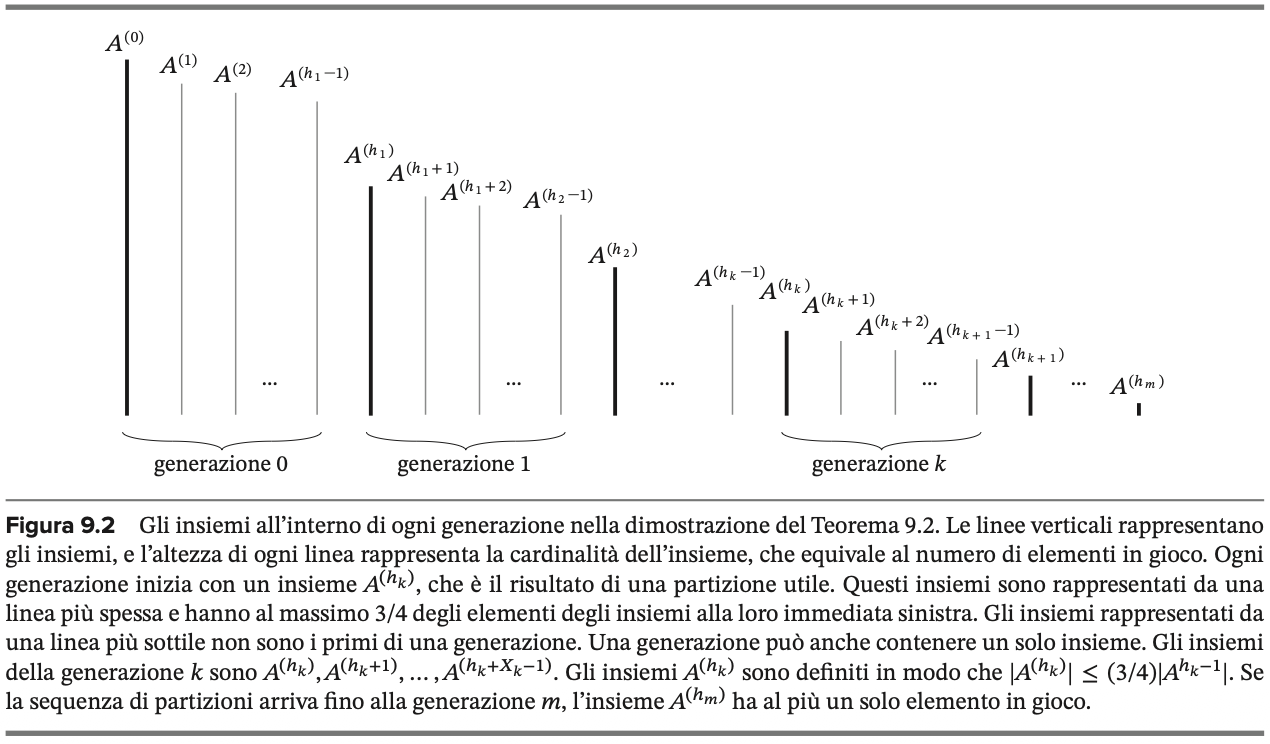
\includegraphics[width=0.75\linewidth]{../images/Screenshot 2026-03-24 alle 00.09.05.png}
    \label{fig:placeholder}
\end{figure}
\noindent Ora definiamo la variabile casuale\\
$$X_k=h_{k+1}-h_k$$\\
per k=0,1,2,..,m-1. Quindi, $X_k$ è il numero di insiemi nella k-esima generazione, di modo che gli insiemi nella k-esima generazione sono $A^{(h_k)}$, $A^{(h_k+1)}$,..,$A^{(h_k+X_k-1)}$.\\
Per il lemma precedente, la probabilità che una partizione sia utile è almeno $\frac{1}{2}$. La probabilità è in realtà maggiore, poiché una partizione è utile anche se il pivot non cade nella metà centrale, ma l'i-esimo elemento più piccolo si torva nella sezione più piccola della partizione. Utilizzeremo comunque la stima inferiore di $\frac{1}{2}$, quindi dall'equazione segue $E[X_k] \le 2$ per $k=0,1,2,..,m-1$.\\
Ne segue che l'equazione di ricorrenza calcolata in precedenza viene al massimo raddoppiata non andando ad impattare sul costo asintotico atteso.\medskip\\
Stimiamo superiormente il numero totale di confronti durante tutte le partizioni. 
Alla $j$-esima partizione si effettuano meno di $|A^{(j-1)}|$ confronti.\\
Raggruppando per generazioni, otteniamo:
\[
\sum_{k=0}^{m-1} \sum_{j=h_k}^{h_k+X_k-1} |A^{(j)}|
\;\le\;
\sum_{k=0}^{m-1} X_k |A^{(h_k)}|.
\]\\
Poiché la dimensione del problema diminuisce geometricamente:
\[
|A^{(h_k)}| \le \left(\frac{3}{4}\right)^k n_0,
\]
segue:
\[
\sum_{k=0}^{m-1} X_k |A^{(h_k)}|
\;\le\;
\sum_{k=0}^{m-1} X_k \left(\frac{3}{4}\right)^k n_0.
\]\\
Prendendo il valore atteso e usando la linearità:
\[
\mathbb{E}\!\left[\sum_{k=0}^{m-1} X_k \left(\frac{3}{4}\right)^k n_0 \right]
=
n_0 \sum_{k=0}^{m-1} \left(\frac{3}{4}\right)^k \mathbb{E}[X_k]
\le
2 n_0 \sum_{k=0}^{m-1} \left(\frac{3}{4}\right)^k.
\]\\
Estendendo la somma a infinito:
\[
< 2 n_0 \sum_{k=0}^{\infty} \left(\frac{3}{4}\right)^k
=
8 n_0.
\]\\
Quindi il numero atteso di confronti è $O(n)$; inoltre, essendo necessario esaminare tutti gli elementi almeno una volta, si ha anche un limite inferiore $\Omega(n)$. 
Pertanto, il tempo di esecuzione atteso di \texttt{RANDOMIZED-SELECT} è:
\[
\Theta(n).
\]
\end{proof}
\section{Selezione in tempo} 
Esamiamo ora un algoritmo di selezione interessante dal punto di vista teorico, il cui tempo di esecuzione è $\Theta(n)$ nel caso peggiore.\\
Come \texttt{RANDOMIZED-SELECT}, che ha un tempo di esecuzione lineare nel caso peggiore, trova l'elemento desiderato partizionando ricorsivamente l'array di input. A differenza di \texttt{RANDOMIZED-SELECT}, però, \texttt{SELECT} garantisce che la partizione sia buona scegliendo, durante la partizione dell'array, un pivot di cui si può provare la bontà. Pertanto ci sono due chiamate di \texttt{SELECT}: una per trovare un buon pivot e una seconda per trovare ricorsivamente la statistica d'ordine.\\
\subsection{Pseudocodice}
prende in input un array A[p : r] di n=r-p+1
 elementi e un intero i tale che $1 \le i \le n$\\
 \begin{verbatim}
1   Select (A,p,r,i)
2   while(r-p+1) mod5 != 0 // operazione di modulo ovvero il resto
3       for j = p+1 to r do
4           if(A[p] > A[j]) then
5               scambia(A[p],A[j]);
6           end
7       end
8       if (i == 1) then
9           return A[p]
10      end
11      p = p+1;
12      i = i-1;
13  end
14  g=(r-p+1)/5;    
15  for j = p to p + g - 1 do
16      ordina_sul_posto(A[j],A[j+g],A[j+2g],A[j+3g],A[j+4g]);
17  end
18  // Cerca ricorsivamente il pivot x come mediana delle mediane
19  x = select(A,p+2g,p+3g-1,(g+1)/2);
20  q = partition_around(A,p,r,x)     //partiziona intorno al  pivot
21  k = q-p+1
22  if(i==k) then
23      return A[q];
24  else
25      if(i<k) then
26          return Select(A,p,q-1,i);
27      else
28            return Select(A,q+1,r,i-k);
29      end  
30  end
\end{verbatim}
\noindent \subsection{Analisi}
\begin{figure}[H]
    \centering
    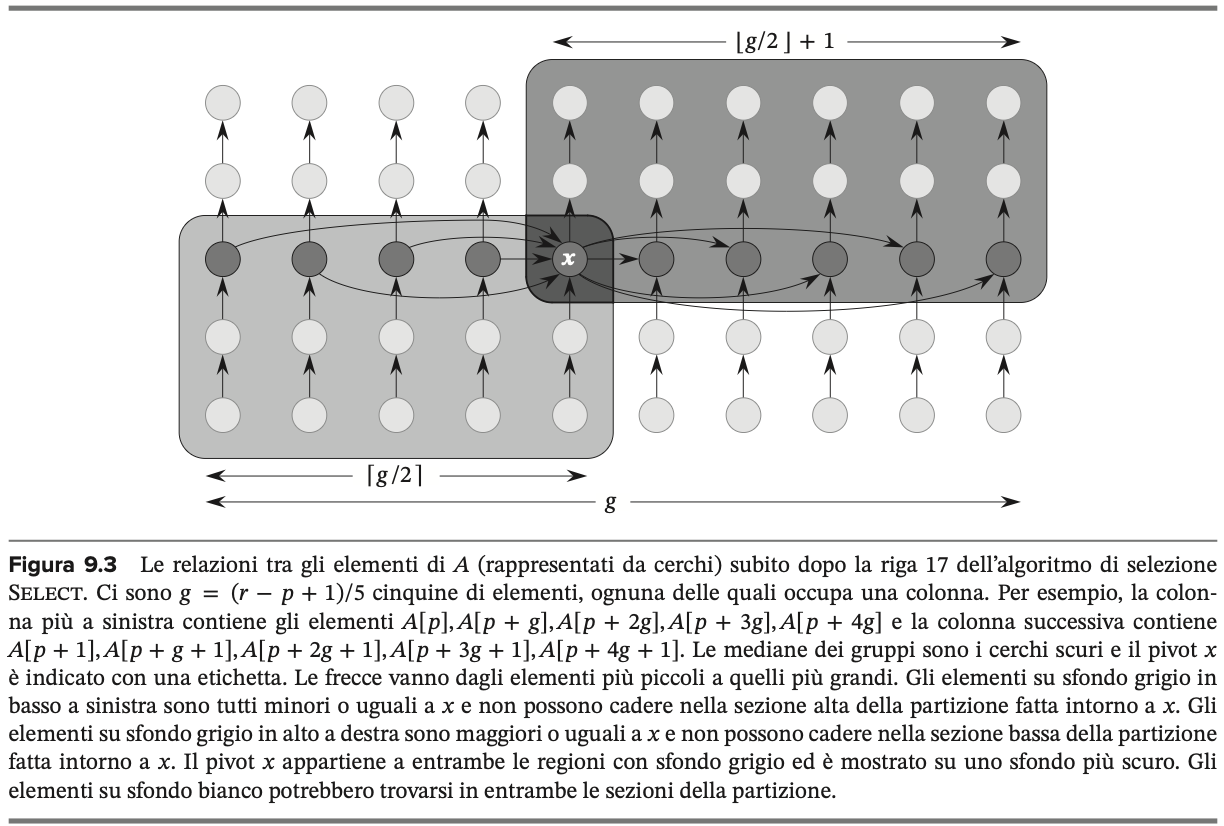
\includegraphics[width=0.75\linewidth]{../images/Screenshot 2026-03-24 alle 19.44.09.png}
    \label{fig:placeholder}
\end{figure}

\noindent Le cinquine sono costruite verticalmente, in modo che gli elementi che le costruiscono siano vicini tra loro. Di ciascuna si seleziona la mediana, con la caratteristica di essere maggiore degli elementi precedenti e minore dei successivi della cinquina. In questo modo si è messo in evidenza l'insieme delle mediane. Con l'istruzione \texttt{x=select(A,p+2g,p+3g-1,(g+1)/2);} si cerca la mediana delle mediane all'interno dell'insieme, questo coincide con l'elemento al centro dell'array complessivo. Una volta chiamata la funzione partiziona questa sposta tutti gli elementi minori di x nel sottoarray di sinistra e quelli maggiori nel sottoarray di destra. Se $i==k$ si è trovata la $k$-esima statistica d'ordine, altrimenti si chiama ricorsivamente la funzione select sul sottoarray di sinistra se $i < k$, o su quello di destra.
